\documentclass[11pt,xcolor={dvipsnames}]{beamer}
\usetheme{Frankfurt}
\usepackage[utf8]{inputenc}
\usepackage[spanish]{babel}
\usepackage{graphicx}
\usepackage{tikz}
\usepackage{amsfonts}
\usepackage{amsmath}
\usepackage{amssymb}
\usepackage{xcolor}
\usepackage{multicol}


\usepackage[super]{nth}
\usepackage{booktabs}
\usepackage{qtree}
\usepackage{commath,soul}
\usepackage{multirow, color, colortbl}
\usepackage{hypcap}

\hypersetup{
    colorlinks,
    citecolor=red,
    filecolor=red,
    linkcolor=red,
    urlcolor=red}



\makeatletter
\newcommand{\srcsize}{\@setfontsize{\srcsize}{3pt}{3pt}}
\makeatother
\logo{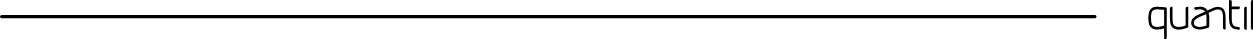
\includegraphics[height=0.34cm]{logo.png}\hspace{20pt}}
\definecolor{quantil}{rgb}{0.33, 0.41, 0.5}
\definecolor{lightseagreen}{rgb}{0.13, 0.7, 0.67}
\colorlet{quantil2}{quantil!59!black}
\colorlet{quantil3}{quantil!40!black}
\setbeamercolor{frametitle}{fg=white,bg=quantil2}
\setbeamercolor{section in head/foot}{bg=quantil3}
\setbeamercolor{author in head/foot}{bg=quantil2}
\setbeamercolor{date in head/foot}{fg=quantil2}
%\setbeamercolor{title}{quantil2}
\setbeamercolor{structure}{fg=quantil2}
\setbeamercolor{section number projected}{bg=lightseagreen,fg=white}
\setbeamercolor{enumerate item}{bg=lightseagreen}
\setbeamercolor{item projected}{bg=lightseagreen}

\AtBeginSection[]{
  \begin{frame}
  \vfill
  \centering
  \begin{beamercolorbox}[sep=8pt,center,shadow=true,rounded=true]{title}
    \usebeamerfont{title}\insertsectionhead\par%
  \end{beamercolorbox}
  \vfill
  \end{frame}
}


%\AtBeginSection{\frame{\sectionpage}}
\AtBeginSubsection{\frame{\subsectionpage}}


\author{Carlos Andrés Reyes}
\title{Reconocimiento de voz (Speech to Text)}
\date{13 de Abril del 2018}

\begin{document}
{ % all template changes are local to this group.
    \setbeamertemplate{navigation symbols}{}
    \begin{frame}[plain]
        \begin{tikzpicture}[remember picture,overlay]
            \node[at=(current page.center)] {
                
\includegraphics[width=\paperwidth]{quantitle.png}
            };
        \end{tikzpicture}
     \end{frame}
}
\begin{frame}
\titlepage
\end{frame}



\begin{frame}{Vocabularios grandes y habla continua (LVCSR)}
\textbf{Objetivo}: Dado un input acústico $O$ encontrar, dentro de todas las frases pertenecientes a un lenguaje L, la más probable.
\begin{itemize}
\item Se divide el input acústico $O$ en intervalos de tiempo (por ejemplo 10 milisegundos) y se trata como una secuencia símbolos individuales:
$$O= o_1, o_2,\ldots, o_t$$.
Cada observación $o_1$ es un vector de features acústicos, en su mayor parte descomposiciones espectrales. 
\item De manera similar se trata una frase como una secuencia de palabras: $$W=w_1,w_2,\ldots,w_n$$
\end{itemize}
$$ \hat{W} = \text{argmax}_{W \in \mathcal{L}}\,P(W\,|\,O) = \text{argmax}_{W \in \mathcal{L}} P(O\,|\,W)\,P(W) $$
\end{frame}

\begin{frame}{Modelos}
$P(W)$: Probabilidad previa, modelo de lenguaje.
\begin{itemize}
\item Modelos N-gram:
$$P(W)= \prod_{k=1}^K P (w_k |w_{k-1} , w_{k-2} , \ldots , w_{k-N +1})$$
\end{itemize}
$P(O\,|\,W)$: Verosimilitud de la observación, modelo acústico.
\begin{itemize}
\item Modelos ocultos de Markov.
\item Modelos acústicos fonemas.
\end{itemize}
\end{frame}

\begin{frame}{Fonemas y alófonos}
\begin{itemize}
\item Son sonidos del habla que permiten distinguir palabras en una lengua. Los sonidos [p] y [b] son fonemas del español porque permiten distinguir palabras como pata y bata que tienen significado distinto y solo diferen en su pronunciación con respecto a estos dos sonidos.
\item A cada fonema corresponden en el habla diferentes sonidos (alófonos) que varian según el sujeto que los pronuncie. 
\item El fonema es un modelo para los alófonos que se efectuan en el habla.
\item Los fonemas son indivisible, no se dividen en unidades menores. 
\end{itemize}
\end{frame}

\begin{frame}{Fonemas y alófonos}
\textbf{Definición formal:} Sea $/f/$ un fonema que puede ser articulado como un conjunto de fonos $\{ \phi_1, \phi_2, \ldots, \phi_n \}$
Se define la función $rasg(\cdot)$ que asigna a cada fono o fonema el conjunto de rasgos relevantes. Entonces se tiene:
$$ \phi_j \in /f/ \Rightarrow rasg(/f/) \subset rasg(\phi_j) $$

Los rasgos están clasificados en las siguientes categorias
\begin{itemize}
\item Principales: silábico, consonático, aproximante, sonorante
\item Laringales: Los estados de la glotis para cada sonido, e.g. sonoro, glotis extendida, constricción glotal.
\item De modo: Continuante, nasal, estridente, lateral, relación retardada.
\item Punto de articulación: Labial, coronal, dorsal, radical, laringal. 
\end{itemize}
\end{frame}
%1
\begin{frame}{Modelo oculto de Markov (HMM)}
\begin{figure}
\centering
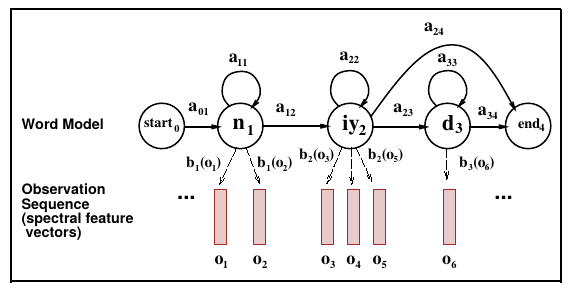
\includegraphics[width=0.7\textwidth]{hmm.png}
\end{figure}
Parámetros que definen un modelo oculto de Markov
\begin{itemize}
\item  \textbf{Estados:} $Q=q_1q_2\ldots q_N$
\item  \textbf{Probabilidades de transición:} $P(x_{t+1}=q_i\,|\,x_t=q_j)= a_{ij}.$
\item  \textbf{Verosimilitud de $o_t$:} $P(o=o_t\,|\,q=q_i) = b_i(o_t)$.
\end{itemize}
\end{frame}

\begin{frame}{Encontrando la secuencia más probable}
Buscamos la secuencia de estados más probable $q^* = (q_1q_2\ldots q_T)$ dada una secuencia de observaciones $o=(o_1o_2\ldots o_3)$.

\begin{figure}
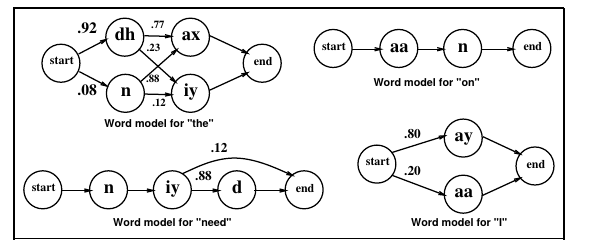
\includegraphics[height=0.35\textheight]{automaton.png}
\end{figure}
\begin{figure}
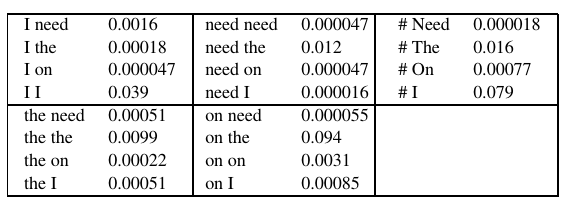
\includegraphics[height=0.2\textheight]{probabilidad_bigramas.png}
\end{figure}
\end{frame}

\begin{frame}{Estructura de pronunciación}
\begin{figure}
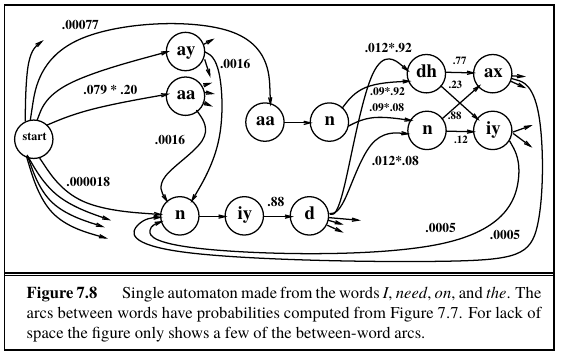
\includegraphics[width=0.8\linewidth]{joined_words.png}
\end{figure}
\end{frame}

\begin{frame}{Encontrando la frase más probable}
\textbf{Algoritmo de Viterbi} Se define la matriz de Viterbi:

$$viterbi[t,i] = \max_{q_1,q_2,\ldots, q_{t-1}} P(q_1q_2 \ldots q_{t-1}, q_t=i, o_1,o_2\ldots o_t\,|\,\lambda )$$
Se llena la matriz de manera recursiva:
$$viterbi [t , j] = \max_i(viterbi[t-1; i] a_{ij} ) b_j(o_t)$$

Se procede al estilo de "Hansel y Gretel" para escoger el camino más probable empezando al final.
\end{frame}

\begin{frame}{Parámetros a entrenar}
\begin{itemize}
\item Modelo de lenguaje: N-gram $P (w_k |w_{k-1} , w_{k-2} , \ldots , w_{k-N +1})$
\item Verosimilitud de las observaciones $b_j(o_t)$
\item Probabilidades de transición $a_{ij}$
\item Léxico de pronunciación: Estructara del grafo de Markov
\end{itemize}
\end{frame}

\begin{frame}{Insumos}
\begin{itemize}
\item Archivos de audio de habla junto con su transcripción en palabras.
\item Un corpus grande de texto para entrenar el modelo de lenguaje, incluyendo las transcripciones.
\item Un corpus más pequeño de archivos de audio marcados fonéticamente. (Los subintervalos son anotados manualmente con sus respectivos fonemas.)
\end{itemize}
\end{frame}

\begin{frame}{Structura gráfica HMM}
\begin{itemize}
\item Se parte de un diccionario de pronunciación
\item Cada fonema del diccionario se mapea a un estado del HMM
\item Estimativo inicial de $a_ij$: Todos los estados son equiprobables. 
\item Estimativo inicial de $b_j(o_t)$: Se estiman a partir del corpus pequeño con anotación fonética. Los modelos gaussianos son menos sensibles a la inicialización.
\end{itemize}
\end{frame}

\begin{frame}{Alineamento forzado de Viterbi}
\begin{itemize}
\item Se toma como input las palabras correctas correspondientes al audio, y los vectores de features del audio.
\item Se forza al algoritmo a a pasar por las palabras con las que se ha marcado el audio. 
\item Se necesita el algoritmo ya que las palabras tienen diferentes pronunciaciones y la duración de cada fonema no es fija. 
\item El resultado es un set de vectores de features acústicos marcados con los fonemas "correctos". Estos se utilizan para reajustar los parámetros de $b_j(o_t).$
\item Para las probabilidades de transición $a_{ij}$ se pueden tomar los conteos de las transiciones en el alineamiento forzoso.
\end{itemize}
\end{frame}

\begin{frame}{Evaluación (Word Error Rate)}
$$ WER = 100\frac{(Inserciones + Supresiones + Substituciones)}{Total\, de \, Palabras}$$
\begin{figure}
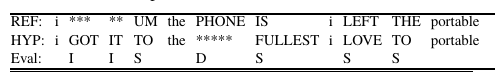
\includegraphics[width=1\linewidth]{errores.png}
\end{figure}
En el 2000 los mejores speech to text tenían un WER del 20\%. Actualmente la mejor evaluación es de Google con 4.9\%.
\end{frame}


{ % all template changes are local to this group.
    \setbeamertemplate{navigation symbols}{}
    \begin{frame}[plain]
        \begin{tikzpicture}[remember picture,overlay]
            \node[at=(current page.center)] {
                
\includegraphics[width=\paperwidth]{gracias.png}
            };
        \end{tikzpicture}
     \end{frame}
}

\end{document}

